%************************************************
\chapter{Discussion}
\label{chp:discussion}
%************************************************

Investigation of fly motion vision provides a compelling example for the methods and goals of systems neuroscience. To extract optic flow from reflected light, the nervous system needs to perform non-trivial but clearly circumscribed computations. Flies accomplish the task using a small number of neurons and within few synapses, suggesting that the project of delivering a circuit-level description of direction-selectivity is indeed tractable. Algorithmic models provide the computational context in which we can embed circuit schemes derived from experimental work. Additionally, motion is a critically relevant stimulus for animals in virtually all ecological niches. Optic flow provides information about our own movement, depth in a visual scene, as well as the movement of conspecifics, prey, and predators. The fact that motion represents such a fundamental cue allows us to put our models of the circuit in the functional context of defined goals.

In the course of this cumulative thesis, my collaborators and I have made substantial progress toward neural models of motion detection in the fruit fly \textit{D. melanogaster}. First, we were able to identify cell groups T4 and T5 as the direction-selective output elements of the ON and OFF motion pathways in the fly optic lobe \citep{Maisak:2013kk}. They form a retinotopic map that delivers locally motion-sensitive signals to the wide-field tangential cells of the lobula plate. Two major functional divisions emerged, one separating contrast polarities and the other concerning directions in visual space. T4 responds only to ON motion defined by brightness increases and T5 only to corresponding OFF motion defined by brightness decreases. Four sub-types of each are selective for only one of the four cardinal directions. When T4 or T5 were silenced, downstream responses both in tangential cells and walking flies were affected in a polarity-specific fashion. In conjunction with the finding that combined silencing of T4 and T5 abolishes all wide-field motion responses, this indicated that the two cell arrays are the dominant source of motion information in the fly brain.

Second, we investigated medulla elements feeding into the T4 pathway \citep{Ammer:2015jo}. Dense reconstruction had suggested a circuit layout in which Mi1 and Tm3 represent the two arms of a Reichardt-type motion detector. Contrary to predictions from this model, only silencing of Mi1 abolished motion responses in tangential cells. Inactivation of Tm3 only had an effect on the specific stimulus regime of fast velocities. Behavioral work confirmed the findings. This ruled out the Mi1-Tm3 model and indicated further neural complexity. Third, we explored this type of architectural complexity in the context of the T5 pathway where we studied the response properties and functional roles of input elements Tm1, Tm2, Tm4, and Tm9 using imaging and genetic silencing \citep{Serbe:2016ew}. These cells provide a broad spectrum of temporal and spatial filters to T5 which are well suited to the computation of motion under a Reichardt-type model. Critically, none of them are themselves direction-selective. When inactivated, physiological and behavioral phenotypes showed that all play a role in OFF motion detection. 

Fourth and finally, having established some of the neural basis of motion detection, we related the emerging two-pathway architecture to its functional context \citep{Leonhardt:2016ex}. In both behavior and physiology, we discovered substantial asymmetries in temporal tuning between the ON and the OFF channel. Simulation work suggested that these asymmetries constitute an adaptation to the particular demands of natural visual statistics. Moreover, they appear to be a critical determinant in the fruit fly's responses to higher-order motion.

\section{A neural model for motion detection}
Key impetus for the projects I pursued during my doctoral studies was the goal of mapping algorithmic elements onto concrete neural implementation. The Reichardt detector and its elaborations have been exceedingly successful at accounting for input-output relationships. Even detailed aspects of optomotor response and neural properties of tangential cells are well predicted by a simple combination of linear filtering and elementary mathematical operations \citep{Borst:1989vp,Borst:2002iw}. It was an open question whether this simplicity would be reflected by neural circuitry. In this section, I discuss correspondences particularly in light of more recent developments.

\subsection{Input lines}
Standard models of local direction-selective units are based on two spatially separated arms that filter visual signals asymmetrically. Work on T4 and T5 inputs, including ours, has hinted at surprising complexity in the presynaptic structure of fly elementary motion detectors. No obvious one-to-one correspondence between algorithm and circuit has emerged. So how should we map neural elements in the medulla onto algorithmic inputs?

\begin{figure}
    \centering
    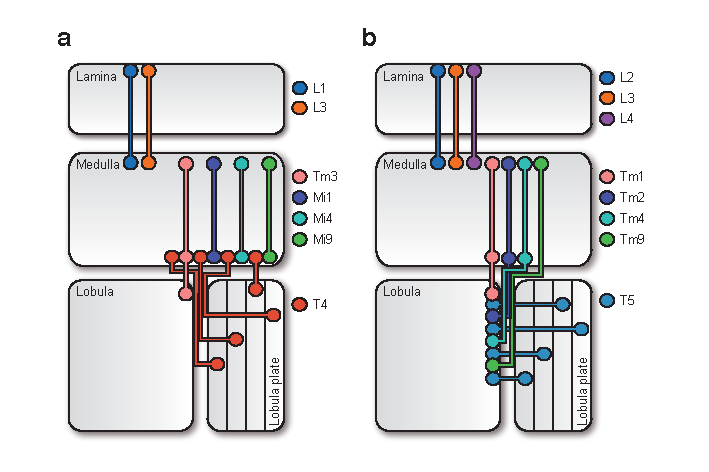
\includegraphics[width=1\textwidth]{graphics/figure_pathway}
    \caption[Map of ON and OFF pathways]
    {Neural architecture of motion pathways based on updated electron microscopy reconstructions. \textbf{a} Schematic of the ON pathway. \textbf{b} Schematic of the OFF pathway. Illustration modified from M.\ Meier with permission.}
    \label{fig:pathway}
\end{figure}

%%%

\subsubsection{ON pathway}
Based on connectivity and a limited spatial offset between projection fields that correlated with the preferred direction of the targeted cell, \citet{Takemura:2013ea} had proposed a two-arm model in which Mi1 and Tm3 relay visual input to the dendrites of T4. There, motion is then computed through a correlation-type mechanism. Electrophysiological recordings from cell bodies of these two cells constrained the model further as the estimated time constant of a filter fit to Mi1 responses was somewhat larger than that of Tm3 \citep{Behnia:2014jh}. Neither Mi1 nor Tm3 were already selective for direction. Together, these findings predicted that input signals are combined on T4 dendrites in a non-linearly opponent fashion as in the model proposed by \citet{Barlow:1965aa}. The correspondence between circuit and a subunit of the Reichardt model would then have been almost one-to-one: starting from photoreceptors, the L1-Mi1 and L1-Tm3 pathways carry a slow and a fast signal, respectively, to the non-linearity implemented by T4.

Several factors detracted from the plausibility of this model. First, the reported difference between filter peaks was approximately \SI{18}{\milli\second} and thus exceedingly small compared to standard values used for modelling of tangential cell responses \citep{Behnia:2014jh}. The steady-state frequency optimum of a simple low-pass Reichardt detector is given by $(2 \pi \tau)^{-1}$ which would require $\tau \approx \SI{150}{\milli\second}$ for the typical post-subtraction peak at \SI{1}{\hertz}. While a direct transfer between time constant and delay shift is not trivial, particularly when the measured filter function is of higher order, the gap is still large. A quantitative model proposed by \citet{Behnia:2014jh} was only able to replicate a well-defined optimum at \SI{1}{\hertz} due to the high-pass characteristics of the measured filters and, importantly, due to the subtraction of oppositely tuned units. Compared to the input signals, output at the subtraction stage was minuscule. Any circuit based on small differences between large signals, however, suffers from a lack of noise robustness. Moreover, the dendrites of T4 already appear to be highly direction-selective but there is now substantial evidence that the subtraction stage is implemented downstream of T4 \citep[see][and the sections below]{Mauss:2015kj}.

Second, the reported separation of the centers of mass of Mi1 and Tm3 projection fields was on the order of \SI{1}{\degree} in visual space, corresponding to only \SI{20}{\percent} of inter-ommatidial distance. While this separation is sufficient to generate direction-selectivity, it again negatively impacts the signal-to-noise characteristics of the resulting circuit. Third, the circuit model clearly predicts that silencing of one input line should abolish direction-selectivity fully. This was not borne out by our findings. Only inactivation of Mi1 affected downstream ON motion responses across the full range of tested stimuli. Note, however, that \citet{Strother:2017aa} found a more completely abolished grating response when imaging T4 in Tm3-silenced flies. Nonetheless, the available evidence pointed toward a more complex circuit layout.

Further studies have recently filled in some of the gaps in our understand of medulla circuitry feeding into T4. The reconstruction effort that had suggested the two-arm Mi1-Tm3 model was subject to methodological constraints that led to an incomplete connectivity matrix. In particular, not all processes impinging on T4 dendrites were followed to their originating columns.

Subsequent work used focused ion beam scanning electron microscopy (FIB-SEM) to image and reconstruct a full cartridge along with its six adjacent columns at a superior voxel size of approximately \SI{10}{\nano\meter} \citep{Takemura:2017aa}. In the resulting circuit diagram, Mi1 and Tm3 were confirmed as major inputs to T4 that jointly represent $\approx\SI{50}{\percent}$ of synapses. The spatial shift between projection fields could not be replicated. Several additional numerically relevant inputs were identified, chief among them Mi4 and Mi9 (complemented by C3, CT1, TmY15, as well as other T4 cells). Dendritic trees of T4 have an elongated structure that covers multiple columns of the medulla and whose orientation correlates with the lobula plate layer to which the sub-type projects. Intriguingly, while Mi1 as well as Tm3 projections tend to target the central area of the dendrite, both Mi4 and Mi9 form synapses in a spatial pattern that depends on the preferred direction of the T4 cell. For upward-sensitive T4c cells, for instance, Mi4 connects primarily on the dorsal end while Mi9 does so ventrally. This yields a mean offset between center and flanking cell of at least one column. This layout and in particular the separation of projection fields between Mi1/Tm3 and Mi4 or Mi9 lend themselves well to Reichardt-type motion computations.

Calcium imaging from these additional medulla cells has critically added to the purely structural view of the T4 circuit \citep{Strother:2014aa,Arenz:2017aa,Strother:2017aa}. As in the OFF pathway, neither of the four inputs is direction-selective by itself which confirms that T4 dendrites are the locus where motion is first extracted \citep{Strother:2017aa}. \citet{Arenz:2017aa} used white-noise stimuli to map spatiotemporal receptive fields and found two transient units which were well-approximated by band-pass filters (Mi1 and Tm3) as well as two tonic units resembling low-pass filters (Mi4 and Mi9). Measurement of step responses yielded comparable results \citep{Strother:2017aa}. An interesting complication arises from the response sign of Mi9. While all other cells increase their calcium levels in response to ON stimulation, Mi9 is activated by OFF stimulation instead. In terms of connectivity, this finds a convenient explanation in the fact that Mi9 lies downstream of OFF-implicated lamina monopolar cell L3. It is conceivable that the synapse connecting Mi9 and T4 effectively reverses the response sign, thereby providing an ON-like signal to T4. Taken together, the filter bank offers a much larger range of temporal properties than what \citet{Behnia:2014jh} had put forward, with time constant differences reaching hundreds of milliseconds. A broad spectrum of course then greatly simplifies the construction of highly direction-selective units.

Given that signals from Mi1 and Tm3 target overlapping parts of the central T4 dendrite and largely come from the same central cartridge, it is a distinct possibility that they interact to form a single functional input arm. There are at least three lines of evidence additionally supporting this notion. First, the FIB-SEM connectome indicates that Mi1 is itself pre-synaptic to Tm3. In fact, Mi1 is the numerically strongest Tm3 input surpassed only by L1. Second, \citet{Strother:2017aa} performed optogenetic activation experiments using UAS-CsChrimson to test functional connectivity between candidate medulla cells and T4 \citep{Klapoetke:2014aa}. Intriguingly, while the isolated activation of Mi1 or Tm3 only had negligible effects on calcium activity of T4 cells, joint excitation of the cell pair resulted in significant signals that were non-linearly amplified over the simple sum of individual responses. Third, our blocking experiments could show that Tm3 plays a critical role in ON motion detection when edge velocities were at the higher end of tested velocities. One could imagine that Tm3 serves to shape and possibly sharpen signals emanating from the central portion of the visual field, in concert with primary projections from Mi1. Silencing of this channel may then only result in clear phenotypes when input dynamics are fast. Overall, the observed complexity highlights that the mapping from circuit to algorithm does not have to be one from single neurons to individual filters and input lines. Individual algorithmic components could well be implemented by a group of neurally segregated units.

\subsubsection{OFF pathway}
Our work on OFF pathway elements paints a similar picture as the one that has now emerged for its ON counterpart. Tm1, Tm2, Tm4, and Tm9 jointly account for a vast majority of the input synapses onto T5 \citep{Shinomiya:2014dx}. None of them are direction-selective, which confines the critical computation to the dendrites of T5. As with Mi1, Tm3, Mi4, and Mi9, they have varying filter properties ranging from the slow and tonic (Tm9) to the fast and phasic (Tm2 and Tm4) with Tm1 showing intermediate kinetics. A Reichardt detector using, for instance, Tm9 and Tm2 as delayed and direct line, respectively, exhibits high direction-selectivity and a frequency optimum in the physiologically plausible range. Conversely, some combinations like Tm2 and Tm4 provided little directional signal, making them unlikely candidates for inputs to the motion detector.

Interestingly, while agreeing on delay direction, we observed a much larger difference between the temporal response dynamics of Tm1 and Tm2 than what \citet{Behnia:2014jh} had reported previously. Possible reasons include calcium kinetics that exaggerate voltage timing differences or asymmetries between measurements in cell bodies and terminals. Note that the Tm2 step calcium responses are indeed slightly faster than the measured voltage deflections.

In our measurements, spatial receptive fields of all T5 inputs were small, isotropic, and retinotopic, with separation and half-width approximately corresponding to what was expected from the facet layout. Additionally, all exhibited lateral inhibition; responses to large stimuli were suppressed. This was later corroborated by filter estimates derived from white-noise responses \citep{Arenz:2017aa}. In contrast, \citet{Fisher:2015aa} employed reverse-correlation and determined receptive fields for Tm9 whose extent was in excess of \SI{60}{\degree} in both elevation and azimuth. The reason for this drastic discrepancy remains unclear. Our work used a different GAL4 line to target Tm9. However, temporal tuning measurements as well as phenotypes in Tm9-silenced flies were in agreement across studies, casting doubt on this explanation. An interesting feature we found when establishing the size tuning of Tm9 using flickering bars of various sizes was an increase in response strength when the bars became large enough to resemble full-field flicker. Through some global pooling mechanism, Tm9 cells appear to have access to information from remote parts of visual space. This observation may be a first step toward reconciling the measurements if one assumes that the measurements by \citeauthor{Fisher:2015aa} were performed in a way that would affect the global properties of the stimulus. For instance, if the recorded terminals have receptive fields close to the borders of the retinotopic map, asymmetric lateral signals may lead to a broadening of the input field of Tm9. From an algorithmic point of view, however, it remains unclear how true wide-field input would critically contribute to direction-selectivity in T5.

The strength of the behavioral phenotypes we found using physiological and behavioral measurements correlated distinctly with the number of synaptic contacts between the respective cell and T5 dendrites. Critically, all four blocks had an impact on downstream motion responses. This lack of redundancy does not indicate a simple division of labor between the potential input arms of the OFF motion detector. In contrast to our work on the ON pathway, temporal tuning curves did not reveal velocity-dependent functional specialization; the reduction in OFF response strength was generally conserved across stimulus frequencies. The strongest effects resulted from blocking Tm2 and Tm9 either individually or in combination. A simple conclusion from this would be to propose Tm2 as the fast and Tm9 as the slow arm of an elementary motion detector. However, this does little to explain the contribution of Tm1 or Tm4 whose silencing, particularly in combination, also produced substantial phenotypes.

\subsubsection{Biophysical origin of delays}
So far, I have tacitly assumed that the temporal filtering of signals reaching T4 is purely intrinsic to the input cells. Given the substantial temporal variety observed at the level of medulla output lines, this is a reasonable assumption.

It is currently not fully understood how medulla cells generate and tune their particular filtering properties. First, it is possible that filter properties are simply inherited from upstream lamina cells. This accounts for a significant fraction of the observed variability. In the OFF pathway, high-pass units Tm1, Tm2, and Tm4 all receive input from the transiently responding L2 \citep{Fischbach:1989uw,RiveraAlba:2011dd,Takemura:2017aa}, with L4 additionally connecting to Tm2. Tonic Tm9 cells, on the other hand, are primarily post-synaptic to L3 for which slow kinetics have been demonstrated \citep{Silies:2013jp}. Within the ON pathway, transient L1 projects to band-pass cells Mi1 and Tm3 while tonic Mi9 lies downstream of L3. Mi4 is targeted by L5 for which photoreceptor input originates from reciprocal connections with L1 (but note that little is known about the intrinsic tuning of L5). Under this scheme, the medulla filter bank is generated by summing lamina output kinetics in various configurations. This provides numerous degrees of freedom. Lamina cells may represent building blocks from which more varied filters can be derived, which attributes interesting functional significance to the multiplexed structure of the fly optic lobe. However, while basic characteristics appear to be derived from upstream processing, further differentiation can be observed. Tm1 and Tm4, for instance, exhibit differing kinetics despite their shared main input L2.

Second, cell-intrinsic mechanisms in medulla pathways could further refine temporal tuning. Passive, purely electrotonic properties of the membrane in neural "cables" produce effects like signal attenuation along appropriately constructed neurites. This results in delays and low-pass filtering of voltage signals that depend on the geometry of processes \citep{Koch:2004aa}. Active conductances along the path may additionally shape signals through, say, non-linear amplification or slow kinetics that introduce temporal offsets. Moreover, synapses represent junction points at which elaborate signal modifications can be implemented through transmission machinery. High-pass filtering, for instance, resembles adaptation. If a synapse removes the long-term mean of the signal by rapid habituation, only sensitivity to fast changes remains. By modulating the kinetics of this adaptation process, different high- or band-pass characteristics are achieved. Adaptive mechanisms have previously been employed to explain phasic output in lamina monopolar cells \citep{Laughlin:1978aa}. Alternatively, high-pass characteristics also emerge when subtracting asymmetrically low-pass filtered signals. This offers yet another biophysically simple mechanism for rendering output transiently sensitive.

It is crucial to note that not all temporal filtering has to be present in the output of medulla inputs. Indeed, the synaptic apparatus connecting them to T4 or T5 may plausibly contribute to the required differential filtering. For instance, there is now evidence from RNA profiling of isolated T4 and T5 cells that these cells express both ionotropic and metabotropic variants of acetylcholine receptors \citep{Shinomiya:2014dx,Pankova:2016aa}. If cholinergic input from one spatial location triggers a slow, muscarinic version and the other a fast, nicotonic version, resulting timing differences may be sufficient to permit the disambiguation of motion direction. More complete neurotransmitter profiles of medulla cells are now available: \citet{Shinomiya:2014dx} propose that all four T5 inputs are cholinergic while findings by \citet{Takemura:2017aa} suggest that Mi1 and Tm3 are cholinergic, Mi4 GABAergic, and Mi9 glutamatergic. This variety offers substantial leeway for synaptic implementations of temporal filtering. Additionally, it is entirely possible that a combination of cell-intrinsic and synaptic mechanisms gives rise to the temporal input profile. Note, however, that the measured cell-intrinsic delays of certain medulla cell combinations appear sufficient to generate strong direction-selectivity \citep{Arenz:2017aa}.

\subsection{Nature of the non-linearity}
The comprehensive mapping of medulla input cells along with the finding that T cell neurites targeting the lobula plate are already selective for direction had revealed T4 and T5 as the locus of the non-linear interaction underlying motion detection. However, the details of this computation remained elusive.

Detailing the neural implementation of a multiplication-like operation has the potential to clarify functional segregation of pre-synaptic elements. After all, input cells clearly outnumber input lines of the Reichardt detector in both pathways. With the exception of velocity-dependence for Tm3, none of the silencing experiments had pinpointed particular functional division among the complex input structure of T4 and T5. The neural non-linearity could shed light on the function of medulla cells.

\subsubsection{Dual mechanisms}
Subunits of the Reichardt detector and Barlow-Levick schemes share the basic principle of differentially delaying spatially adjacent signals and then comparing them in order to establish temporal order. Where they differ is the choice of non-linearity that implements comparison. For the Reichardt detector, this is correlation as realized by mathematical multiplication. Large output signals occur when two inputs are in phase after one of them is delayed. For Barlow-Levick detectors, the essential operation is an AND-NOT gate. Only inputs with appropriate phase relationships pass; signals resulting from null motion are vetoed. The two layouts make clear predictions about the placement of the delay as well as the input-output signature of the operation that combines inputs. One of them is fundamentally facilitating; the other one is fundamentally suppressive.

Several studies have now made progress toward a neural understanding of the operations implemented by fly motion-sensitive neurons. First, \citet{Fisher:2015jo} used apparent motion to discriminate excitatory and inhibitory interactions on dendrites of genetically singled-out T4 and T5 cells. When stimulated with spatially neighboring, temporally separated flashes along the cells' preferred direction, T4 dendrites showed direction-selective calcium increases that exceeded the linear prediction calculated from the sum of responses to isolated flashes. The same facilitating response was observed for T5\footnote{Interestingly, \citet{Fisher:2015jo} also reported a non-linear suppression of responses to apparent motion along the null direction but discarded this as motion-unselective adaptation.}. This indicated that the non-linear interaction on both T4 and T5 dendrites is based on the amplification of coincident signals, in line with what the Reichardt model had predicted.

Second, \citet{Leong:2016hu} used system identification methods to fit T5 white-noise responses. Given the inherent non-linearity of direction-selective responses, they built a cascade that consisted of chained linear (L) receptive fields and point non-linearities (N), forming a LNLN feedforward model that also modelled calcium binding dynamics. Such a phenomenological model contrasts with mechanistic accounts like the Reichardt detector. As expected and in line with the internal structure of motion energy models, response variance was best explained by a spatiotemporally slanted receptive field combined with polynomial non-linearities of orders 3 and above. Within the linear spatiotemporal filter, two spatially separated sub-fields could be identified: one with positive sign, one with negative sign. The authors interpreted this as a dual mechanism for generating OFF-specific direction-selectivity that recruits both facilitation and suppression. Note, however, that their method does not allow for conclusive disambiguation of, say, ON facilitation and OFF suppression.

Third and finally, \citet{Haag:2016cq} probed the dendritic non-linearity through a combination of precisely targeted apparent motion and layer-specific read-out of T4 activity. The former was accomplished by telescopic stimulation of isolated neuro-cartridges; the second by expressing the calcium indicator under the control of a T4c-exclusive driver line. Single T4 cells have elongated receptive fields that span multiple columns. When apparent motion consisting of ON illumination steps was focused on the center, both non-linear amplification of preferred direction sequences as well as non-linear suppression of null direction sequences could be observed. This demonstrated explicitly that both mechanisms underlie direction-selectivity on T4 dendrites. Critically, at the dorsal and ventral end of the receptive field only suppression and facilitation, respectively, occurred. This indicated a clear functional division among input elements at opposite ends of the dendritic tree.

\begin{figure}
    \centering
    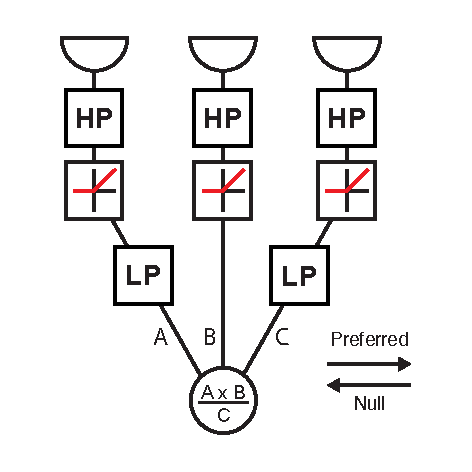
\includegraphics[width=0.55\textwidth]{graphics/figure_models2}
    \caption[Combining Reichardt and Barlow-Levick detectors]
    {Simplified schematic of signal flow in the three-arm detector for T4 motion responses as proposed by \citet{Haag:2016aa}. Input stages resemble the previous two-quadrant iteration, with high-pass filtering being followed by half-wave rectification. Input B mediates a fast central signal. Inputs A and C supply delayed facilitating and suppressing signals, respectively. Note that for reasons of simplicity, the DC contribution is omitted in this illustration.}
    \label{fig:detector2}
\end{figure}

In concerts, these studies argue in favor of a synthesis of Reichardt and Barlow-Levick models. The biological algorithm draws from three visual inputs to implement both an excitatory and an inhibitory non-linearity. \citet{Haag:2016cq} put forward a simple extension of the standard correlation scheme in which the output of a multiplicative Reichardt sub-unit is divided by a third spatially displaced input, effectively creating a serial circuit consisting of two half-detectors. In this model, the central arm is a fast line and the flanking inputs contain appropriate delays. The model mimics T4 responses to apparent motion closely and produces plausible frequency tuning curves.

Importantly, it resolves a puzzling observation for T4 and T5 measurements that were part of our initial functional characterization. Sub-units of Reichardt detectors show little direction-selectivity by themselves; they generally respond vigorously to motion in both preferred and null direction. Only after subtraction do responses become unambiguously sensitive to one or the other. Our initial assumption was that T4 and T5 are ON- and OFF-specific half-detectors as in the two-quadrant model suggested by \citet{Eichner:2011ic}. However, both neurons exhibited remarkable selectivity for direction when stimulated with gratings or edges. That is, responses of T4 and T5 sub-types were sharply tuned to one direction in visual space and suffered from little off-target activation. The three-arm detector provides a consistent explanation for this property: if enhancement of preferred stimuli and suppression of non-preferred stimuli act in concert, crisp tuning follows even at the level of half-detectors. This architecture ensures high signal-to-noise ratio alrady at the local stage that precedes subtractive or spatial integration. Given the data by \citet{Leong:2016hu} and follow-up work using telescopic stimulation (Jürgen Haag, personal communication), it is probable that motion extraction in T5 relies on a comparable dual non-linearity.

The elaboration of the correlation detector also contextualizes the input complexity that our work on T4 and T5 inputs has suggested. A motion detector of this type requires at least three arms, which reduces the number of seemingly extraneous input cells to just one. Moreover, given their relative spatial displacement, T4 inputs Mi1/Tm3, Mi4, and Mi9 now map neatly onto central and peripheral lines of this novel architecture. Taking this as well as temporal filter properties into account, \citet{Arenz:2017aa} could show through simulations that a detector in which Mi4 acts as a delayed facilitating input, Mi1 as a fast central input, and Mi9 as a delayed inhibitory input exhibits high direction-selectivity. Finally, T4 inputs release a wide spectrum of neurotransmitters including glutamate, acetylcholine, and GABA \citep{Takemura:2017aa}. This offers opportunity for post-synaptic receptors to realize various non-linear interactions.

Due to a lack of dense reconstructions that trace processes back to the medulla, our understanding of how Tm1, Tm2, Tm4, and Tm9 synapses cluster on T5 dendrites is fundamentally limited \citep{Shinomiya:2014dx}. This hinders the mapping between cells and input lines of a three-arm detector. Quantitative work based on their filter properties finds that the best performing three-arm detectors have Tm2 as the fast central arm, Tm9 as the slow inhibitory arm, and either Tm1 or Tm4 as the facilitating arm \citep{Arenz:2017aa}. It is noteworthy that the OFF pathway appears to lack a second true low-pass filter next to Tm9. This poses a challenge when constructing parallel correlation detectors. Curiously, all T5 inputs appear to be cholinergic. While it is possible that acetylcholine receptor diversity is sufficient to realize differential non-linearities, further RNA profiling efforts could revise this picture in the future.

\subsubsection{Neural implementation}
The exact nature of both facilitating and suppressing non-linearity currently awaits detailed investigation. A standard Reichardt detector uses full multiplication to correlate incoming signals. Motion-energy models rely on output of the form $(a+b)^2$ which of course implicitly contains the product of inputs $2ab$. Some studies have analyzed the spectral properties of tangential cell responses to local grating motion, assumed to only stimulate individual motion detector units, and concluded that the comparison is indeed almost perfectly multiplicative, with little contribution from higher-order non-linearities \citep{Egelhaaf:1989wf}.

From a biophysical point of view, it is unlikely that individual neurons compute sign-correct multiplication. This would require excessively complex synaptic machinery. Even at the algorithmic level, however, the problem can be transformed to become more tractable without losing essential properties of multiplication. The \textit{Drosophila} visual system, for instance, reduces implementation complexity by only considering two quadrants of the full operation, namely the multiplication of equally signed ON-ON or OFF-OFF inputs \citep{Eichner:2011ic}. Each non-linearity then operates on appropriately half-wave rectified positive signals and produces exclusively positive output. Similar tricks have successfully been applied to the design of analog electric circuits \citep{Mead:1989aa}. In the context of looming sensitivity in giant locust neurons, \citet{Gabbiani:2002kb} proposed a straightforward decomposition of the product $ab$ into the exponentiation of summed log-transformed inputs, $\exp(\log a + \log b)$. Both logarithmic response curves and exponentiation through active conductances are of course common response features of real neurons \citep{Koch:2004aa}. Null direction inhibition, on the other hand, could plausibly be achieved through linear summation of appropriately signed inputs followed by application of a threshold.

We can additionally imagine various molecular ways in which excitatory or inhibitory coincidence detection could be implemented. To be sensitive to temporal order, two sets of channels need to be linked in a causally asymmetric manner. Consider a piece of membrane in which the delayed input targets a metabotropic, G-protein coupled receptor and the direct input an ionotropic receptor. If the cascade downstream of the metabotropic receptor renders the ligand-gated ion channel more sensitive, then preferred direction stimuli result in non-linearly amplified cation flux through the second channel. This ultimately depolarizes the cell. Out-of-sequence stimulation still produces potentials but at substantially smaller magnitude. Alternatively, the G-protein cascade is replaced by a ligand-gated calcium channel; within the cell, these ions then modulate the sensitivity of the secondary input. Vetoing of signals for the suppressive arm could rely on ligand-gated anion channels that realize a type of divisive or shunting inhibition. For a tractable electric model of how this may be achieved, see for instance \citet{Torre:1978vp}.

In the case of motion detection, many different types of non-linear interactions result in similar outcomes. Note, however, that the exact properties of facilitation and suppression are not necessarily mere implementation details. \citet{Fitzgerald:2015aa}, for instance, demonstrate that elaborations of the non-linear step of correlator models yield improvements in velocity estimation performance for natural scenes. Our own work on response asymmetries represents a concrete example in the fruit fly visual system. Here, the reduced implementation of multiplication in separate ON and OFF channels provides additional degrees of freedom for precise tuning to realistic statistics.

\subsection{Integration of signals}
Following non-linear interaction, Reichardt-type models of both tangential cell and optomotor responses contain multiple stages of integration. First, oppositely tuned half-detectors are subtracted from each other. Second, a large number of adequately weighted local detectors is summed to produce a global estimate of optic flow. Subtraction in particular greatly enhances the direction-selectivity of resulting output, but note that combined facilitation and suppression on T4/T5 dendrites already improves signal quality in the half-detector \citep{Borst:1990wu,Haag:2016cq}. While generally depicted in this order, linearity ensures that the exact sequence does not matter.

Integration of local information on the finely tuned dendrites of tangential cells is well understood due to extensive work in larger flies \citep{Borst:2010fk}. Our characterization of T4 and T5 added another stage to this circuit layout. Up to the lobula plate where tangential cells pool the output of hundreds of input neurons of both types, motion information remains segregated into polarity-specific ON and OFF channels. Only then do these processing streams merge. Models generally assume that this summation is approximately linear; see for instance the two-quadrant detector outlined above. Yet, it is entirely conceivable that a more complex combination of polarity-selective signals occurs. For typical flow fields generated by ego-motion, ON and OFF motion are strongly correlated. Consider moving your head toward the left in front of a spatially confined dark object. In the reference frame of the retina, this object moves toward the right. Direction signalled by its leading dark edge is precisely correlated with trailing bright edge motion, simply due to rigidity of the scene. Integration mechanisms could take advantage of such correlations when globally combining ON- and OFF-derived flow. Whether this speculation has any grounding in physiological reality and how this could be exploited, however, remains to be seen.

Subsequent work has clarified the neural substrate of subtractive motion opponency. In a first study, \citet{Mauss:2014is} used whole-cell patch clamp to monitor the potential of tangential cells while optogenetically activating the full array of T4 and T5 cells. They observed a biphasic response that consisted of fast depolarization followed by delayed and prolonged hyperpolarization. Through pharmacological intervention, the excitatory potential could be identified as cholinergically mediated while chloride conductances appeared to underlie inhibitory potentials. In sum, these findings strongly suggested that T4 and T5 neurons from one layer provide excitatory input to LPTCs while corresponding units from the oppositely tuned layer produce null direction hyperpolarization via some inhibitory interneuron. This fit well with the finding that T4 and T5 are cholinergic \citep{Raghu:2011iy,Shinomiya:2014dx,Pankova:2016aa} and excluded the hypothesis that unidentified secondary units provide null direction signals computed \textit{de novo}.

These intermediaries have since been identified as glutamatergic lobula plate-intrinsic (LPi) neurons \citep{Mauss:2015kj}. They exhibit appropriate connectivity from oppositely tuned layers, produce inhibitory potentials in tangential cells upon optogenetic activation, respond to motion in a predictably tuned fashion, and are critically necessary for null direction-driven LPTC hyperpolarization. Using a variety of visual stimuli, it was possible to show that their action confers drastically enhanced flow field selectivity to downstream sensors \citep[see][]{Krapp:1996}. Given that hyperpolarization of LPTCs is unlikely to control behavioral output, this may represent a key justification for opponent wiring at this level.

An interesting observation from studies on tangential cell responses was the asymmetry between preferred and null direction tuning, with the latter generally being weaker than the former \citep{Egelhaaf:1989wf,Joesch:2008fo}. Various models including the two-quadrant detector have incorporated incomplete motion opponency to explain, for instance, residual flicker responses \citep{Eichner:2011ic}. Physiologically, this may be due to the activation threshold of LPi neurons. Its functional significance remains unclear.

%%%

\subsection{Emergence of polarity-selectivity}
Our initial calcium imaging experiments on lobula plate terminals of T4 and T5 had indicated that when stimulated with edges, both are strongly selective for polarity. OFF edge responses in T4, for instance, were drastically smaller than corresponding ON edge responses, but some residual cross-polarity activity was observed. It was not clear whether this was due to insufficiently specific GAL4 lines or if it did indeed reflect imperfect separation of ON and OFF. We were later able to show that when imaged in medulla or lobula where T4 and T5 do not intermingle, cross-polarity responses are indeed zero. This poses an interesting question. The visual system operates on photoreceptor input that encodes both brightness increases and decreases. The final product of the motion detection system is strongly half-wave rectified. Where does this selectivity arise, and how is it achieved?

\subsubsection{Neural level}
Some evidence has pointed toward the lamina. Sharp-electrode recordings from monopolar cells in large flies reveal a high-pass filtered signal that depolarizes for OFF and hyperpolarizes for ON. The calcium level of L1 and L2 axon terminals in \textit{Drosophila} is transiently responsive to both negative and positive changes in luminance, but there are indications of amplitude asymmetries in L2 that favor OFF stimuli as would be expected for inputs to the pathway terminating in T5 \citep{Reiff:2010eo,Clark:2011gw}. High-pass filtering followed by transmission of only positive or negative changes is a simple recipe for ON-OFF splitting. For instance, if pre-synaptic calcium channels in lamina projection neurons only open upon depolarization and remain closed for hyperpolarization, then transmitter release to downstream cells is restricted to one polarity. Yet, more sustained lamina cells like L3 have been implicated as input elements to both ON and OFF motion computation, suggesting that signal rectification is not complete at the earliest level of pathway separation \citep{Silies:2013jp,Takemura:2017aa}.

Moreover, medulla cell recordings paint a somewhat fuzzy picture. In line with expectations and with only one exception (Mi9), response signs of signals are transformed by intermediate synapses such that ON pathway cells are activated by brightening stimuli and OFF pathway cells by darkening stimuli. \citet{Behnia:2014jh} estimated rectification by fitting a linear-nonlinear cascade model to white-noise voltage responses of Mi1, Tm3, Tm1, and Tm2. Critically, none exhibited strong polarity-specificity. This was reflected by subsequent simulations. When putting empirical filters of, for instance, Mi1 and Tm3 into a Reichardt detector model, only mild selectivity for edge polarity was observed. This contrasts with our findings in T4 and T5 and suggests additional mechanisms. For instance, the non-linear step in T4 and T5 could be implemented in a way that enhances half-wave rectification. Moreover, \citet{Yang:2016aa} compared membrane potential and calcium concentration under visual stimulation using genetically encoded indicators for both. They observed that calcium activity of motion-related medulla cells was more selective for ON or OFF than electrical activity, implicating the transformation between the two in the implementation of half-wave rectification.

Our measurements of OFF pathway input cells yielded three cells whose calcium activity was insensitive to ON edge stimulation. Tm9, however, encoded low-pass filtered brightness changes in both directions through increases and decreases of calcium levels. This demonstrates that information about both polarities remains available at the level of medulla terminals, which is further emphasized by the subsequent finding that one ON pathway cell increases its calcium levels for OFF stimuli \citep{Arenz:2017aa,Strother:2017aa}. Moreover, the degree of rectification appears to depend on the particular stimulation regime tested, with continuously varying stimuli like white-noise generally producing smaller asymmetries between ON and OFF response magnitudes than step inputs \citep{Reiff:2010eo,Clark:2011gw,Behnia:2014jh,Arenz:2017aa}. We quantified selectivity for polarity by stimulating with locally step-like edges. It would thus be worthwhile to additionally explore separation using other stimulus dynamics.

%%%

\subsubsection{Algorithmic level}
The question of rectification also affects quantitative descriptions of motion detection circuits. The two-quadrant model as proposed by \citet{Eichner:2011ic} implemented pathway separation through high-pass filtering (or pseudo-differentiation) of positive brightness signals, adjustment of the response sign for ON or OFF subunit, and subsequent half-wave rectification to remove information about the other direction of change. This layout modeled response properties of L1 and L2 and corresponding silencing experiments effectively \citep{Laughlin:1978aa,Joesch:2010fw} but requires modifications in light of the updated circuit scheme. Given the filtering properties and strong blocking phenotype of Tm9, for instance, it is likely that a pure low-pass filter feeds into the T5 non-linearity. L3 is thought to supply tonic signals to both pathways \citep{Silies:2013jp,Takemura:2017aa}. Overall, the input structure appears to be much less delineated than anticipated. To maintain polarity selectivity after the non-linearity while incorporating knowledge about the multi-input structure, additional rectification steps seem to be required.

Fly reverse-phi phenomena are yet another factor in need of reconciliation. Robust responses to spatiotemporal correlations of ON and OFF can be observed in tangential cells \citep{Egelhaaf:1992wh,Eichner:2011ic} and optomotor behavior \citep{Tuthill:2011ic,Clark:2011gw}. In the two-quadrant detector, this is resolved by allowing for a small and positive tonic luminance component to feed into both subunits \citep[see also][]{Kern:2000a}. Interactions at the border of apparent motion steps, for instance, then result in negative responses for mixed-polarity combinations. Additionally, DC can account for retained sensitivity for apparent motion that is separated by extreme durations of more than \SI{10}{\second}, which exceed estimated neural time constants by orders of magnitude \citep{Eichner:2011ic}. My optimization experiments using natural images revealed that limited DC enhances velocity estimation performance. Interestingly, this improvement was largely independent of scene statistics. It is possible that DC sensitivity adds to the robustness of output for noisy stimuli; minor ON-OFF interactions could mediate a noise cancellation mechanism that attenuates the impact of non-linearly amplified fluctuations. Neural evidence for retained DC sensitivity even in the responses of transient lines like Mi1 or Tm3 exists \citep{Behnia:2014jh}. Additionally, our measurements in the OFF pathway as well as subsequent work clearly demonstrate the presence of tonic inputs to both T4 and T5, such as Tm9 or Mi4.

The DC model of reverse-phi responses appears to be in conflict with our observation that for edge stimulation, no cross-polarity responses occur for either T4 or T5. Given the minor weight of tonic sensitivity, it is possible that responses for the opposite edge polarity are too small to trigger calcium channels. Using voltage indicators to study sub-threshold events in T4 or T5 could provide critical evidence. In any case, the problem of how to reconcile polarity selectivity and reverse-phi output awaits further investigation and modelling work.

\subsection{Sources of asymmetry}
Both edge velocity tuning measured in tangential cells and optomotor responses elicited by a balanced edge stimulus confirmed that the two \textit{Drosophila} motion pathways differ in temporal tuning. Optimal OFF edge velocities substantially surpass peak ON edge velocities. We could show that this was not due to electrophysiological consequences of differential adaptation state. The neural basis of these asymmetries is currently not clear. \citet{Behnia:2014jh} had shown similar delays for the two cell pairs they tested. However, it is now evident that T4 and T5 each derive motion-critical inputs from at least four input cells. These filter arrays provide numerous degrees of freedom for shaping velocity tuning. Depending on how the non-linearity combines inputs, a broad range of velocity optima is possible. Indeed, when \citet{Arenz:2017aa} calculated temporal tuning for three-arm detectors based on all possible input combinations, they found that reasonably direction-selective T5 models had slightly higher peak frequencies than corresponding T4 models. Due to uncertainty about the exact division of labor among the numerous T4 and T5 inputs as well as the biophysical implementation of the non-linearity, however, we can currently not yet pinpoint the exact mechanisms that give rise to a particular velocity tuning.

Measurements of T4 and T5 velocity tuning have so far not revealed tuning asymmetries as they are clearly observed in downstream tangential cells. Our own data indicate a temporal frequency optimum of $\approx \SI{1}{\hertz}$ for both channels. Differences in stimulus statistics may contribute to these discrepancies. The transformation of inputs up to motion-selective stages is unlikely to be purely linear, so temporal characteristics could well be different for step-like edges when compared to dynamic noise or patterns like sine-wave gratings. Under this model, asymmetries would only emerge under particular stimulus conditions. Yet, \citet{Arenz:2017aa} determined edge velocity tuning curves for T4 and T5 and found little evidence for asymmetries. It is possible that small tuning differences are amplified through summation subsequent to initial motion computation. For instance, T4 and T5 responses peak for very slow edge velocities below \SI{10}{\degree\per\second}; only spatiotemporal integration shifts them into the range of \SIrange{100}{300}{\degree\per\second} which is observed at later stages.

\subsection{Further elaborations}
Recent inquiries into the neural circuitry of fly motion vision, including the studies that comprise this thesis, have made significant headway toward a neurally plausible model of how direction-selectivity arises. Nonetheless, critical question marks remain. First, our algorithmic models are pure feedforward systems. There is substantial evidence in favor of multiplexed feedback from downstream stages modulating the activity of lamina, medulla, and lobula plate \citep{Fischbach:1989uw,Takemura:2017aa}. For instance, silencing lamina feedback neurons Lawf2 specifically alters the lower range of temporal frequency tuning in flight optomotor responses \citep{Tuthill:2014gc}. It is possible that such projections are primarily useful for state-dependent modulation of response properties, but blocking feedback neurons C2 and C3 has been shown to affect the visual detection of gap width in exploring flies \citep{Triphan:2016aa}. Feedback may conceivably underlie aspects of computation, so future investigations will have to incorporate these projections into their models of the circuit.

Lateral connections are currently equally under-explored. Our OFF pathway characterization of input neurons shows that most units are size-tuned, suggesting lateral inhibition. Indeed, spatial filters estimated from white-noise responses generally consist of an excitatory center and a subtractive surround \citep{Arenz:2017aa}. For the L2 pathway, some of this processing may already originate in the lamina \citep{Freifeld:2013gu}. It is unclear whether lateral effects are purely subtractive or whether non-linear normalization also occurs. An interesting data point comes from Tm9 which shows size-tuning as well as substantial full-field flicker responses. It is possible that non-linear, potentially divisive lateral inhibition is responsible for this effect \citep{Carandini:2012fma}. Anatomical mapping of the medulla offers several candidate cells whose ramifications span multiple columns \citep{Fischbach:1989uw}. Elaborate signal normalization could help to explain the peculiar contrast tuning exhibited by tangential cell responses and optomotor behavior when stimulated with natural images. Here, artificially imposed global changes in scene contrast but not natural contrast variation strongly modulates the amplitude of responses \citep[see our work as well as][]{Straw:2008hh}. This could be due to mechanisms that locally adjust the neuron's operating range.

\section{Comparative views}
\subsection{Parallels to other visual systems}
Motion detection represents a fundamental computation that underlies a multitude of behaviors in many species. Remarkably, work on the optomotor response in beetles and an investigation of direction-selectivity in the rabbit retina have both resulted in similar correlation-based algorithmic models, the Reichardt and Barlow-Levick detectors respectively \citep{Hassenstein:1956fa,Barlow:1965aa}. It stands to reason that not only phenomenology but also mechanism is conserved across animals. In the following section, I briefly discuss similarities between invertebrate and vertebrate motion vision at the level of neural implementation.

Genetic accessibility has made fruit fly and mouse the key targets of investigations tackling peripheral motion vision \citep[for thorough reviews, see][]{Borst:2015ko,Euler:2014aa}. The mammalian retina is a layered, retinotopically organized structure that consists of photoreceptor layer, outer nuclear layer, outer plexiform (synaptic) layer, inner nuclear layer, inner plexiform layer, and a ganglion cell layer. Light is transduced by two types of photoreceptors, cones and rods, which primarily but not exclusively specialize in day- and nighttime vision, respectively. Interestingly, the structure of the retina is anatomicallly "inverted" with respect to processing direction: incoming light passes all layers before it reaches the innermost receptor layer. Unlike the fly photoreceptor, rods and cones hyperpolarize in response to brightness increases. This means that in the absence of light, they constantly release glutamate (giving rise to the term "dark current"). The crucial downstream cell types are horizontal, bipolar, amacrine, and ganglion cells. Bipolar cells are the critical relay between photoreceptors, which they contact in the outer plexiform layer, and ganglion cells, which they contact in the inner plexiform layer. Through the optic nerve, axons of the latter project to various downstream areas, including the lateral geniculate nucleus from which visual signals reach cortex.

At the level of bipolar cells, a crucial parallel between invertebrate and vertebrate systems emerges. As in lamina and medulla of the fly optic lobe, signals become separated into ON and OFF channels. OFF bipolar cell dendrites express glutamate-gated ion channels that depolarize the cell for brightness decreases. For ON bipolar cells, a metabotropic glutamate receptor reverses the sign of responses and thus depolarizes the cell for brightness increases. Bipolar cell projections in the inner plexiform layer are then stratified according to the transmitted contrast polarity. Bipolar cells implement substantial multiplexing of signals across at least 13 identified sub-types. This resembles the large number of retinotopic medulla channels in the fly visual system. Almost each of these bipolar cell types densely tiles the retina, forming a grid that determines the system's spatial resolution. Ganglion cells generally pool from multiple bipolar cells, rendering the grid somewhat coarser, and can be subdivided into a large number of types based on anatomy and function. Recent high-throughput classification attempts, for instance, have identified more than 35 functionally distinct classes \citep{Baden:2016aa}. 

Within the outer plexiform layer, inhibitory horizontal cells mediate lateral interactions at the level of the photoreceptor-bipolar synapse. Similarly, inhibitory amacrine cells within the inner plexiform layer provide lateral connectivity among ganglion cells. The latter can roughly be divided into small-field glycine-releasing and wide-field GABA-releasing units.

At least three retinal ganglion cell types spike in a direction-selective fashion: four sub-types of ON-OFF cells, each sensitive to a single cardinal direction; three sub-types of ON cells, which divide visual space into three equally spaced directions; and invariably upward-selective OFF JAM-B cells. So-called starburst amacrine cells are critically required for motion extraction in the ON-OFF type and have been found to be direction-selective themselves, with their preferred direction running from soma to tip of their circular dendritic tree. Interestingly, this radial arrangement means that starburst cell compute motion along many more possible directions than T4 or T5 which sample only four cardinal directions through their four appropriately aligned sub-types.

Starburst cells are now thought to be the stage where a delay-and-compare strategy is implemented, hinting at a further parallel to T4 and T5 cells in the fly visual system. Bipolar cell projections to the inner plexiform layer show a broad range of response kinetics, with slower characteristics dominating at the fringe of ON and OFF layers and faster responses being prevalent toward the center \citep{Baden:2013ir}. This bears a striking resemblance to the spectrum of temporal filters we measured for OFF input cells as well as more recent work on the full set of ON input cells \citep{Arenz:2017aa,Strother:2017aa}. Assuming that faster bipolar cells synapse with starburst cells near their dendritic tips while slower inputs connect close to the soma, an appropriate non-linearity could render the amacrine cells direction-selective. Indeed, reconstruction efforts have uncovered spatially precise connectivity that matches this scheme \citep{Kim:2014aa} which implies that a Reichardt-type facilitation scheme underlies direction-selectivity in these cells. When comparing it to the fly, this layout lines up well with the elongated, multi-columnar structure of T4 dendrites as well as the spatial specificity of synapses made with differentially filtered input lines \citep{Takemura:2017aa}.

In visual cortex, direction-selectivity is found in structures as early as V1 and propagated downstream to integration areas where increasingly abstract representations and global estimates of optic flow are computed \citep[for a review of motion-critical primate area MT, see][]{Born:2005aa}. This processing stream could be construed as paralleling the pooling that occurs in the fly lobula plate. However, flow field sensitivities of fly tangential cells appear tightly coupled to particular visuomotor reflexes, casting doubt on the notion of abstraction. There is no clear consensus to what degree motion is computed \textit{de novo} in the cortex, but evidence points toward a complex mixture of newly generated and retina-inherited motion responses \citep{CruzMartin:2014aa}.

\subsection{ON and OFF processing}
The separation of changes in sensory magnitude into increases and decreases is a leitmotif of the thesis at hand. Throughout the four collected studies, I have investigated both how and why this split occurs, all in the context of fly motion vision. Employing simulations and experiments, we were able to demonstrate that ON and OFF channels in \textit{Drosophila} are differentially tuned and that these asymmetries may reflect tuning to natural stimulus statistics. Of course, the division of ON and OFF represents a ubiquitous principle that spans modalities and species. Examples include thermosensation in fruit flies \citep{Gallio:2011aa}, olfactory processing in \textit{C. elegans} \citep{Chalasani:2007aa}, auditory processing in the rat \citep{Scholl:2010aa}, and electrosensation in fish \citep{Clarke:2015aa}. Moreover, separation of ON and OFF has been demonstrated in visual systems ranging from flies \citep{Joesch:2010fw} over mice \citep{Euler:2014aa}, cats \citep{Wassle:2004aa}, and primates \citep{Field:2007aa} to humans \citep{Hashimoto:2013aa}. The sheer universality makes it likely that polarity-specific sensory computation confers general advantages that go beyond the requirements of isolated tasks.

First, I have discussed above that the biophysical implementation of a non-linearity that can compute ON-ON and OFF-OFF motion in one step would require exquisitely complicated physiological machinery. After all, this operation demands that very different inputs (for instance, positive and negative changes in membrane potential) result in identical output. If incoming signals are restricted to one direction of possible change per pathway, the task reduces to a significantly more tractable problem. The fundamental problem of correlating bipolar signals is of course not restricted to motion vision. Barn owls, for instance, localize potential prey based on minute phase differences between acoustic signals impinging on their ears. This mechanism is highly similar to how Reichardt-type models extract motion. There is strong evidence that coincidence detection of differentially delayed signals supports this ability in the owl \citep{Jeffress:1948aa,Carr:1988aa}. Separate processing of ON and OFF can also simplify such computations for other modalities.

Second, given the implementation cost incurred by a dual-pathway architecture, one may wonder why it is insufficient to just extract motion for one of the two polarities. As mentioned above, in most environments optic flow as generated by ego-motion around various body axes results in substantial ON as well as OFF motion. Visually confined objects, for instance, are usually represented by contrast changes of both contrast polarities at their leading and trailing edges. Tangential cells would then be able to extract reasonably reliable flow fields from just T4 or T5 activity. However, the two motion pathways feed into multiple behaviorally relevant downstream circuits whose demands could well differ. A prominent example is the visually mediated escape response. Approaching objects or landmarks---in contradistinction to entities traveling sidewards---produce looming optic flow that is defined by only one expanding edge polarity. Only if ON and OFF motion are extracted does the fly retain the ability to evade both bright and dark predators. In line with this, experiments have shown that T4/T5 block flies lose their ability to steer away from expanding stimuli \citep{Schilling:2015jh}. Generally speaking, animals cannot afford to neglect approximately \SI{50}{\percent} of all available sensory input.

Third, the natural statistics of any sensory modality can be shaped in a way that results in asymmetries between the two polarities. In this case, separate processing gives the brain an opportunity to tailor response properties to the particular demands of dark and bright stimuli. Our own work on fruit fly motion vision offers one such example where differential temporal tuning appears to confer an adaptive advantage when estimating the velocity of a rigidly translating natural image. The causally relevant skewness of luminance in the real world also affects other visual tasks, so it is a distinct possibility that ON/OFF asymmetries in other visual systems serve a similar function. \citet{Chichilnisky:2002wu}, for instance, observed timing differences, asymmetric levels of rectification, and varying receptive field sizes between ON and OFF retinal ganglion cells in the primate retina. Interestingly, they found OFF cells to slightly lag their ON counterparts. A plethora of studies has now accumulated substantial evidence for functional asymmetries between ON and OFF in vertebrate systems \citep{Zemon:1988aa,Zaghloul:2003aa,Jin:2011aa,Yeh:2009aa,Pandarinath:2010hg,Copenhagen:1983aa,Burkhardt:2011aa,Gollisch:2008jv}. Physiologically, a difference in temporal kinetics between ON and OFF responses originates immediately at the level of photoreceptor synapses. OFF bipolar cells receive input via fast ionotropic receptors while ON units rely on slower metabotropic receptors. Remarkably, there is evidence that these asymmetries persist up to the level of visual cortex and even perceptual decisions, so a functional role seems probable \citep{Komban:2014cq}. Most of these studies used flash stimuli and did not specifically focus on motion processing in retina or cortex. It will be interesting to see whether the specific asymmetries we report transfer to other species. In general, the task-centric perspective could shed light on why functional differences propagate to higher processing stages.

Fourth and finally, considerations from information theory provide a principled reason for why dual-channel processing is preferential. To code changes in both directions of interest using a single output, sensory cells have to maintain intermediate activity levels even in the absence of salient stimuli. \citet{Gjorgjieva:2014ks} studied the information transmission in either single polarity systems consisting of two ON units or a mixed ON-OFF configuration. Interestingly, both exhibited identical maximum information rates when constraining their peak firing rate. However, the ON-OFF system did so with substantially fewer spikes. The observed gain was multiplied when the stimulus distribution contained rare but large events. A key advantage of separate ON and OFF processing may therefore be metabolic efficiency, which constrains all sensory systems.

\section{Behavioral investigation of neural circuits}

One of my core contributions to the papers of this cumulative thesis was work on genetically manipulated walking fruit flies. Behavioral assays enjoy a long tradition in circuit neuroscience, going back to the cyberneticists in the tradition of von Uexküll, Wiener, and many others. Teasing apart the rules that govern an organism's behavior through observations of input-output relationships offers a principled way of studying information-processing systems. However, it is also subject to severe limitations, particularly when aiming for a level of neural grounding. The genetic methods outlined in the introduction and used throughout the main part have greatly improved this aspect of behavioral experiments. In the following section, I discuss various pitfalls and advantages of the behavioral approach as applied to sensory neuroscience.

\subsection{Visuomotor transformations}
My chief interest throughout my doctoral work was the algorithmic and neural structure of the elementary motion detector in \textit{Drosophila}. Behind the approach taken lay the assumption that the optomotor response of walking or flying flies represents a reasonably close read-out of the activity in upstream circuits close to the sensory periphery. To a certain extent, this supposition holds. As seen in the exposition, motion-driven locomotion faithfully recapitulates many response features of LPTCs or T4 and T5 activity like tuning to temporal frequency or dependency on contrast. However, it is essential to note that the output of local motion detectors goes through a complex and lengthy cascade of additional processing steps.

There is now significant evidence for the causal link between tangential cell responses and subsequent motor output. Early lesion studies and experiments on mutants with abnormal lobula plate elements were able to show that resulting optomotor deficits were severe and specific \citep{Heisenberg:1978aa,Geiger:1981aa,Hausen:1983js}. Naturally, these manipulations were too coarse to establish precise links between particular LPTCs and behavioral capability. Recently, genetic experiments on GAL4-targeted tangential cells have advanced the state of the art. As for sufficiency, \citet{Haikala:2013cm} demonstrated that optogenetic activation of HS cells in the fruit fly elicits yaw head and body movements in tethered flying flies whose sign depends on the stimulation side in a predictable manner. With regard to necessity, \citet{Kim:2017aa} used UAS-Kir2.1 to disrupt signalling in HS and VS cells and found head motion responses to be completely abolished. Interestingly, they only observed a partial reduction of motion-dependent wing beat differences. This hints at additional complexity and may implicate additional sets of LPTCs.

While lobula plate output appears critically required for the optomotor response, LPTCs are not true pre-motor neurons; signals are further filtered, gated, and gathered by downstream stages. A substantial of our knowledge concerning the connections between optic lobe and motor circuits controlling walking or flying comes from studies of large flies \citep{Strausfeld:1985aa,Strausfeld:1990aa,Haag:2007ir,Wertz:2008jt}. It is now clear that many aspects of the layout of downstream projections is indeed conserved in the fruit fly \citep[for instance, see][]{Suver:2016aa}. In addition to projections to head motor systems, axons of lobula plate neurons ramify in the so-called posterior slope of the central brain. From here, neurons target the thoracic ganglion and ventral nerve cord. These parts of the nervous system house the motor control centers that guide whole-body steering efforts. Indirect lobula plate projections form but a small part of the estimated \SI{1100} descending neurons \citep{Hsu:2016aa}.

There is ample evidence that the machinery acting post-LPTC implements non-trivial processing as part of the visuomotor transformation. For \textit{C.\ vicina}, \citet{Wertz:2009hb} could show that descending neurons of the ocellar and vertical system (DNOVS) render the coding of optic flow associated with particular body rotations more robust when compared to their upstream inputs, VS cells. Non-linear gating through other sensory modalities like wind as well as behavioral state was revealed by experiments on visual properties of ventral cervical nerve motor neurons \citep{Haag:2010fy}. In the fruit fly, \citet{Suver:2016aa} suggest that a set of DNOVS-like descending neurons computes specific linear combinations of VS and HS inputs and are directly associated with stereotyped motor programs. Yet another example for presumably motion-driven descending neurons is the giant fiber neuron that triggers rapid evasive take-offs in response to looming \citep{Reyn:2014aa}. Finally, the mapping between sensorimotor and flight muscle commands indicates remarkable multiplexing into large phasically active actuators that mediate rapid strong turns and small tonically active actuators that mediate continuous small-scale turning \citep{Lindsay:2017aa}.

For models of elementary motion detection derived from behavioral assays, this poses a challenge as visuomotor processing may well affect our conclusions about peripheral sensory mechanisms. However, past success justifies the approach: despite the apparent complexity, simplistic approximations of the visuomotor transform like linear spatial integration have enabled the development of influential models like the Reichardt detector \citep{Hassenstein:1956fa}. Such black-box models have proven intriguingly adept at explaining even earliest stages of computation. Critically, early sensory networks act as bottlenecks. Many fundamental tuning properties are thus necessarily inherited by the ensuing cascade that gives rise to motor commands. Particularly in combination with genetic approaches, we can use the optomotor response as a powerful high-throughput read-out of detector activity and draw conclusions about mechanisms of direction-selectivity. Behavioral experiments in this thesis have generally replicated tangential cell phenotypes; the velocity-specific impairment following Tm3 block is a noteworthy example.

\subsection{State dependencies}
Flies are dynamic animals that navigate a dynamic world. For reasons of both efficiency and effectiveness, sensory systems ought to adjust their properties to current behavioral demands. This implies that the visual system of the fly is not a static feedforward processor. State-dependencies severely complicate the investigation of visual mechanisms, especially when using behavioral tools for circuit mapping. Expectations about visual statistics affect fly behavior at several temporal timescales. Our work on adaptation through tuning asymmetries presumably operates on the slowest, evolutionary ones. In the following, I discuss short-term modulation.

\subsubsection{Fast adjustment}
\textit{Drosophila} flight is separated into at least two locomotor motifs: straight continuous flight and rapid saccades. For most of the flight duration, flies maintain straight heading. Course control then relies heavily on fast adjustments of trajectory; within dozens of milliseconds, flies turn at an approximately right angle, easily reaching speeds of thousands of degrees per second \citep{Mronz:2008eb,Straw:2011eua,Muijres:2014aa}. Interestingly, body saccades appear to be both spontaneous and elicitable by visual input \citep{Tammero:2002aa,Mronz:2008eb,Censi:2013cya}. Saccade-like high-velocity turning is observed even in tethered flight. For the optomotor system, they pose a problem. If the fly for instance aims to voluntarily turn to the right, the resulting visual following reflex would directly counteract the saccade and keep it on an unintended straight course.

Several solutions for this challenge have been devised. First, the frequency optimum of the optomotor response may alleviate the effect of the optomotor response. If the yaw rotation is sufficiently fast, resulting optic flow exceeds the sensitivity of the motion detector and no response is generated. However, natural scenes have significant power in the range of lower spatial wavelengths; even at high turning velocities, residual reflexive locomotion could hamper the fly's ability to reorient. Second, an influential model for how stabilizing feedback loops can be reconciled with voluntary perturbation is the notion of efference copies, which goes back to von Helmholtz. The optomotor reflex represents a simple control loop that mitigates deviations from a set point. By taking into account the sensory feedback that is expected from a motor command when computing these deviations based on sensor signals, internally and externally controlled factors can be differentiated. Indeed, \citet{Kim:2015kr} described motor-related potentials in LPTCs whose sign and timing were such that they would cancel visual signals generated through saccade-like voluntary turns. There are now indications that these potentials do not represent a blanket shutdown of all LTPC activity for the duration of the saccade. Instead, they appear to be precisely targeted to the lobula plate units for which any given flight maneuver would produce undesireable output \citep{Kim:2017aa}. Other tangential cells remain unaffected and able to suppress the effect of external perturbations.

\subsubsection{Slow timescales}
Behavioral modes critically influence the expected visual statistics. The average velocity of rotational optic flow, for instance, greatly differs between rest, walking, and flight. To maximize the impact of the optomotor system and avoid saturation, motion circuits should adjust their operating range depending on the current state of the animal. A fundamental observation with regard to such modulations is the almost tenfold difference between frequency optima determined in LPTCs of immobile flies and walking or flying animals \citep{Joesch:2008fo,Duistermars:2007aa}.

A multitude of studies has tracked state-dependent visual properties in the fly optic lobe. \citet{Chiappe:2010cl} used calcium imaging to measure frequency tuning curves in HS cells of fruit flies walking on a treadmill set-up. During walking LPTC responses increased drastically, particularly at high frequencies. In a closely related study, \citet{Maimon:2010jy} recorded from VS cells during tethered flight. Activity boosted response gain through a lowering of passive membrane resistance. LPTCs in large flies are subject to similar modulations of temporal response curves, especially at high stimulus frequencies expected during flight \citep{Jung:2011bc}. Intriguingly, the latter study was able to mimic the active behavioral state via ectopic application of an octopmaine agonist, CDM. This neurotransmitter appears to be the crucial mediator of state throughout the fly nervous suystem. \citet{Suver:2012bya} could alter temporal tuning by silencing or activating octopaminergic projection neurons.

Intriguingly, the effects of state modulation are measurable even at early stages of visual processing \citep{Arenz:2017aa}. After CDM is applied, both T4 and T5 and their medulla input cells shift their sensitivity toward higher stimulus frequencies. Temporal filter properties of all tested inputs sped up. This is not entirely surprising: in a correlation-based model, velocity tuning is not affected by response filtering subsequent to the non-linearity that gives rise to direction-selectivity. Nonetheless, it is an impressive demonstration for the malleability and flexibility of sensory circuits in the fly.

More generally, the finding that even the periphery is affected by behavioral variables casts doubt on the notion that sensory and motor processing is separable at a neural level. LPTCs are often described as matched filters for optic flow that feed into visuomotor circuits. However, there are strong indications that HS cells additionally encode an estimate of walking speed \citep{Fujiwara:2017aa}. Given these data, it appears that the fly optic lobe is better described as a visuomotor area than a purely visual one. This design principle is sensible when considering the minuscule size of the fly brain. If the number of neurons is limited, early specialization and maximized relevance for behavior are advantageous. Note that research on mice has uncovered motor signals in primary visual cortex \citep{Keller:2012aa,Saleem:2013aa}, so significantly larger brains appear to be subject to similar constraints.

\subsection{Motion detectors as feedback sensors}
As mentioned above, optomotor responses implement a stabilizing system that prevents course deviations through visual feedback \citep{Goetz:1965aa}. In an import sense, motion-sensitive elements in the lobula plate thus act as the sensors of a simple controller, signalling the error that downstream motor command centers attempt to reduce. During our simulations as part of the investigation of ON/OFF asymmetries, we used a tractable objective function to optimize the performance of the Reichardt-type model: correlation between the velocity of a rigidly translating visual scene and average detector output. 

At the surface level, this seems sensible; a reliable estimate of true rotational velocity allows for precisely controlled countermeasures. However, we did not analyze optimality in the context of a dynamical system like the optomotor feedback controller. \citet{Warzecha:1996bm}, for instance, studied stabilization behavior of tethered flying flies in artificial visual environments and argued that non-proportional velocity tuning helps stabilizing the feedback loop by suppressing large oscillations. Constraints of this type only emerge in closed-loop settings. It would be of interest to optimize detector parameters in a feedback regime and compare results to the open-loop tuning we performed.

Feedback controllers are prevalent throughout many engineering disciplines. A particularly popular approach makes use of so-called PID controllers \citep{Astrom:2008aa}. They base their corrective output on three parallel signals: one proportional to the current error; one that integrates the error and thus guarantees that the system approaches zero for constant deviations; and one that differentiates the error, which effectively implements a type of predictive counteraction. There is substantial evidence for proportional and little for anticipatory or differential control in the fly. \citet{Schnell:2014hs} recently suggested that integration of motion-evoked calcium levels occurs in the terminals of HS cells. This clashes with our observation that walking flies do not fully counteract their externally imposed offset from straight heading in closed-loop experiments. If the corrective signal was truly integrative, steady-state deviations should eventually go to zero. It seems conceivable that the observed effects are due to strong temporal low-pass filtering.

The relationship between LPTC response and magnitude of the locomotor output appears to be strongly amplifying: even small depolarizations or "errors" can result in substantial turning vigor. This transfer function ensures that the feedback controller has appropriate gain even under adverse signal conditions. However, it may well mask silencing phenotypes if the block is not absolutely complete. Residual tangential cell activity then permits virtually unchanged behavioral output. Yet, using appropriately designed stimuli the robustness of the transformation can be put to use by exploiting the machinery to amplify the phenotype of interest. Throughout the studies of this thesis, I employed balanced motion stimuli \citep[modified from][]{Clark:2011gw} that consisted of ON and OFF edges drifting in opposite directions at the same velocity. LPTC signals are zero in case of equally strong ON and OFF responses. Only when the two channels diverge do motion responses arise. Even small phenotypes are then amplified by the compressive transfer function. This way, we were able to detect ON/OFF asymmetries as well as phenotypes induced by silencing of T4 and T5 input cells. Indeed, the amplification effect may even confer increased sensitivity over direct LPTC measurements; a subtle velocity-specific effect was observed when blocking Tm2, which disproportionally affected higher velocities compared to Tm1, Tm4, and Tm9. Moreover, comparing the magnitudes of tangential cell and behavioral block phenotypes for the OFF pathway allowed us to quantify the transformation in detail and revealed a clearly non-linear relationship.

\subsection{Post-hoc approaches}
All experimental work I applied to the problem of motion detection were fundamentally interventionist in nature. By varying visual input in concert with targeted genetic manipulations, we were able to characterize response properties and build models in a forward manner. Laboratory experiments always run the risk of distilling artificial behavioral motifs or pushing neural circuitry into synthetic regimes that do not reflect ethological function \citep{Krakauer:2017aa}. As mentioned in the introduction, our causal interventions determine what we get out. Just like in Plato's cave, we only see a particular projection of the system. This projection may or may not reflect the system's true nature.

Recently, the ethological, fundamentally post-hoc perspective has gained traction once more \citep{GomezMarin:2014aa}. This is greatly simplified by state-of-the-art methods for observing, recording, and analyzing complex behavioral sequences. Advances in machine learning have been particularly important for this development as they allow the rigorous, possibly less biased extraction of patterns in high-dimensional representations \citep[for instance, see][]{Kabra:2013aa}. \citet{Branson:2009aa} analyzed \textit{Drosophila} behavior in a high-throughput screen by applying statistical methods to time-resolved walking traces. Interestingly, it was possible to identify the genotypes of flies purely based on these observations. It would be worthwhile to apply these methods to motion-guided visual behavior. This may simplify the search for neural candidates involved in processing and even support model building.

\section{Outlook}
In the course of my work on fly motion vision, we made substantial progress toward a neural understanding of optomotor behavior and investigated how this polarity-specific circuitry is shaped by its natural context. The emerging neural layout exhibits intriguing complexity, with a larger than expected number of cells shaping the responses of elementary motion detectors. Fly motion vision therefore represents a compelling example for the incredibly intricate interplay between neural processing systems and their environment.

From here on, several lines of inquiry suggest themselves. First, exact functional division among T4 and T5 input cells remains unclear, with many hypotheses being based on mere compatibility. The combination of high-precision read-outs like telescopic stimulation and genetic silencing of individual input neurons may yield further insight into the mechanisms that produce preferred direction enhancement and null direction suppression. Molecular and physiological investigation of the functional properties of synapses that connect input arms to T4 or T5 dendrites will be equally critical in this endeavor. Recent innovations in the design of genetically encoded voltage indicators could further illuminate the sub-threshold processes that give rise to direction-selectivity. Finally, optogenetic activation has shed some light on non-linear interactions between T4 inputs \citep{Strother:2017aa}. Artificial induction of realistic motion responses using patterned illumination would be a significant step toward a mechanistic understanding, putting a physiological spin on the idea that we do not understand a system until we can build it ourselves.

Second, at the behavioral level, a broadening of the range of stimuli used to probe the optomotor response is required. During our characterization of Mi1 and Tm3 as well as Tm1, Tm2, Tm4, and Tm9 we only scanned a single parameter, pattern velocity. In the OFF pathway, this was of course motivated by the differential temporal tuning we had observed in calcium responses. However, it is possible that functional separation runs along other factors such as luminance or contrast. This may be particularly relevant for the question of why there are more than three input cells per pathway; a potential modulatory function of the fourth arm could be restricted to specific input regimes.

Third, we focused on velocity estimation when optimizing detector parameters in the context of temporal asymmetries between ON and OFF. The activity of elementary motion detectors is likely to underlie various tasks other than the optomotor response like looming-triggered escape or even depth perception \citep{Schilling:2015jh,Schwegmann:2014ir}. Exploring the constraints imposed by other tasks could help to grasp the complexity of the \textit{Drosophila} optic lobe. It is testament to the elaborate intricacies of even the minuscule fly brain that despite all progress, we are not running out of things to investigate.